\documentclass[9 pt]{book}

\usepackage
{
	tikz,
	pgfplots
}

\usetikzlibrary{trees}

\begin{document}

\section*{Class One}
\subsection*{Statistics {\tiny Discipline}}
\hspace{4 mm} Statistics is the discipline that concerns the collection, organization, analysis, interpretation and presentation of data for any policy purpose. In applying statistics to a scientific, industrial or social problem, it is conventional to begin with a statistical population or a statistical model to be studied. Statistics deals with every aspect of data, including the planning of data collection in terms of the design of surveys and experiments. So, we can say, statistics is a mathematical body of science that pertains to the collection, analysis, interpretation of explanation and presentation of data as a branch of mathematics. Some consider statistics as a distinct mathematical science rather than a branch of mathematics.

\subsection*{Data}
Data is the information comes from observations, measurements, counts and responses.

	\begin{itemize}
		\item[\textbf{Observation} $\rightarrow$] \textit{That things obtained by only observation {\tiny(Sit back and watch what's going on)}, no need to count or measurement.}
		\item[\textbf{Measurement} $\rightarrow$] \textit{Data that needs to be measure. Such as height, weight etc.}
		\item[\textbf{Count} $\rightarrow$] \textit{Data that needs to be count to collect / store. eg. how many patients are waiting in queue.}
		\item[\textbf{Response} $\rightarrow$] \textit{The information we obtain from that question which ans either yes or no.}
	\end{itemize}
	
{\large O}kay, that's pretty good. There are two types of data (According to collection method):-\linebreak

	\begin{center}
		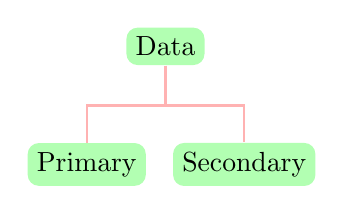
\begin{tikzpicture} [sibling distance=20mm, level distance=15mm, edge from parent fork down, every node/.style={fill=green!30, rounded corners}, edge from parent/.style={red!30, thick, draw}]
			\node {Data}
					child {node {Primary}}
					child {node {Secondary}};
		\end{tikzpicture}
	\end{center}
	
	\begin{itemize}
		\item[\textbf{Primary}] data are the information recorded as a part of the original study. When data required for a particular study can be found neither in the internal records of any organization nor in the published sources. It may become necessary to collect original data to conduct first hand investigation.\linebreak
		Methods for primary data collection:-
			\begin{enumerate}
				\item[\textbf{Observation Method:}] In an observational data collection method, you acquire data by observing any relationships that may be present in the phenomenon you are studying. There are four types of observational methods that are available to you as a researcher:-
					\begin{enumerate}
						\item Cross-sectional
						\item Case-control
						\item Cohort
						\item Ecological
					\end{enumerate}
			\end{enumerate}
		\item[\textbf{Secondary}] When you collect data after another researcher or agency that initially gathered it makes it available, you are gathering \textbf{secondary data}. Such as, census data. One advantage to using secondary data, it saves time and money. Although, some data sets require you to pay for access. Collect secondary data may assume a shortcut way of information gathering.
	\end{itemize}
	
\end{document}
